\documentclass{llncs}
\usepackage[utf8]{inputenc}
\usepackage[english]{babel}
\usepackage{hyperref}
\usepackage{wrapfig}
\usepackage{proof}

\pagestyle{plain}

\newcommand{\liquidsoap}{Liquidsoap}
\newcommand{\savonet}{Savonet}
% Il ne s'est rien passé ici...
\newcommand{\eg}{\emph{e.g.},}
\newcommand{\ie}{\emph{i.e.},}
\newcommand{\cf}{{cf.~}}
\newcommand{\TODO}[1]{\marginpar{\tiny #1}}
\newcommand{\ignore}[1]{}
% useless space around captions
\newcommand{\fcaption}[1]{\vspace{-3ex}\caption{#1}\vspace{-4ex}}

\newcommand{\sub}{<:}

\usepackage{graphicx}
\usepackage[matrix,arrow,frame]{xy}

\usepackage{tikz}
\usetikzlibrary{snakes}

\title{\liquidsoap{}:\\
  a High-Level Programming~Language\\
  for Multimedia~Streaming}
\author{David Baelde\inst{1} \and Romain Beauxis\inst{2} \and Samuel Mimram\inst{3}}
\institute{
  University of Minnesota, USA
  \and
  Department of Mathematics, Tulane University, USA
  \and
  CEA LIST -- LMeASI, France
}

\hypersetup{
  pdftitle={\csname @title\endcsname},
  pdfauthor={David Baelde, Romain Beauxis and Samuel Mimram},
  unicode=true,
  colorlinks=true,
  linkcolor=black,
  citecolor=black,
  urlcolor=black
}

\hyphenation{pa-ra-me-trized}

\begin{document}
\maketitle

% \vspace{-4ex}

\begin{abstract}
  Generating multimedia streams, such as in a webradio, is a task which is
  complex and difficult to adapt to every users' needs. We introduce a novel
  approach in order to achieve it, based on a dedicated high-level functional
  programming language, called \emph{\liquidsoap{}}, for generating,
  manipulating and broadcasting multimedia streams. Unlike traditional
  approaches, which are based on configuration files or static graphical
  interfaces, it also allows the user to build complex and highly customized
  systems. This language is based on a model for streams and contains operators
  and constructions, which make it adapted to the generation of streams. The
  interpreter of the language also ensures many properties concerning the good
  execution of the stream generation.
  % We describe a model that supports a rich collection of operators (track
  % scheduling, jingle insertion, mix, metadata updates, various transitions), and
  % some aspects of language design that make it adapted to the application
  % domain.
\end{abstract}

The widespread adoption of broadband internet in the last decades has
changed a lot our way of generating and transmitting information. Classical
devices from the analog era, such as television or radio broadcasting devices
have been rapidly adapted to the digital world in order to benefit from the new
technologies available. Whilst analog devices were mostly based on hardware
implementations, their digital counterpart often consists in software
implementations,
% , \eg{} hardware
% PBX for phone communications being replaced by software like Asterisk and IP
% phones.
which potentially offers much more flexibility and modularity in their design.
% and allow updates, both for bugfix and new features, at virtually no cost.
% In this context of improvements, updates and enhancements of old technologies,
% we are here specifically interested in adapting audio and video broadcasting
% techniques to the digital world.
% So, creating and broadcasting a stream of multimedia data with recent computers
% has become technically very easy.
However, we believe that the current software technologies to perform such tasks
have not yet fully brought the new ideas which are necessary in order to really
benefit from the new possibilities offered by modern computing devices.

We are specifically interested here in the generation of multimedia streams
(containing audio or video). For example, many webradios are continuously
broadcasting audio data streams, and people can connect to these in order to
listen to the radios. At first, generating the streams might seem really simple:
it is just a bunch of concatenated audio files. However, in practice the needs
of real-world radio makers are much higher than this, and designing a generator
for multimedia streams needs a lot of flexibility in order to be able to cope
with most of the expectations and requirements of users. For instance, a radio
stream may have jingles announcing next coming shows or commercials. It may also
play those jingles at a regular interval of time, between songs or on top of
them. Also, a radio program may be composed of automatic playlist for a certain
period, \eg{} during the night, and live shows during the day. Similarly, one
may want to control and process the data before broadcasting it to the public,
performing tasks like volume normalization, cross-fading between tracks
(possibly parameterized by the respective volumes of the old and new tracks or
predefined settings), blanks removal (nobody wants to listen to silence),
etc. Moreover, the generation of the stream should be rock-solid: most webradios
are broadcasting automatically 24/7 and don't want to have to manually restart
the generator if it crashes after a few hours or a few days.

Those examples, among many others, show the need for very flexible and modular
solutions for creating and broadcasting multimedia data. Most of the currently
available tools to broadcast multimedia data over the Internet (such as Darkice,
Ezstream, VideoLAN, Rivendell or SAM Broadcaster) consist of straightforward
adaptation of classical streaming technologies, based on
predefined interfaces, such as a virtual mixing console or static file-based
setups. Those tools, although quite powerful, are usually very hard to adapt to
a particular need and are more and more often perceived as limited by the very
\TODO{DB "new" c'est abusé}
\TODO{RB c ok avec innovative ?}
constrained design of the program. Here, we present an innovative methodology for
achieving the task based on a dedicated \emph{programming language} called
\emph{Liquidsoap}, which brings much more flexibility and has proved in practice
to be adapted to the needs of a wide variety of users' requirements.

Programming languages are a particularly important aspect of modern software
technologies.  Whether general or domain-specific, programming languages are
often the right tool to release creativity and flexibility for creating new
applications. They have been used in various practical contexts to bring
flexibility and overcome static pre-defined paradigms. One may, for instance,
think of Perl, invented to allow powerful and flexible word-based treatments, or
PHP, which allows to easily create dynamic web pages. We believe that a good
programming language should follow three fundamental principles: it should be
\begin{enumerate}
\item \emph{adapted}: users should be able to perform, most of the tasks in the
  domain of application of the language (generating multimedia streams in our
  case);
\item \emph{simple}: users should be able to perform the tasks in a simple way
  (this means that it should be reasonably concise, but also reasonably
  understandable -- keep in mind that people willing to generate webradios are
  far from being all good programmers);
\item \emph{safe}: the compiler should perform checks to avoid as many bugs as
  possible (a stream generator has for example to ensure that there will always
  be data to stream).
\end{enumerate}
Designing a programming language that fulfills these requirements is not an easy task.
Since the concept is quite new for the generation of streams, a
lot of time was spent to identify the needs of potential users, and to find the
right constructions and operators to build streams. The description of these is
one of the main interests of the paper: we both detail the abstract model for
streams underlying our software, and describe the actual programming language
\liquidsoap{}. Interestingly, we have been able to reuse and adapt classical
techniques and tools for programming languages, which turn out to fit and be
quite natural in this context: the language \liquidsoap{} is functional (which
confers a lot of expressiveness to it) and strongly typed (which allows to have
strong guarantees on the behavior the stream generation).

The aim of the article is to present not only the programming language
\liquidsoap{}, but also the solutions that had to be found for problems which
are specifically raised by to our domain of application. We first give a broad
overview of the language and its underlying model of streams in
Section~\ref{sec:liq}. We then illustrate the typing system and the need for
dedicated constructions in order to type multimedia streams in
Section~\ref{sec:content}. Finally, we describe in Section~\ref{sec:clocks} the
problems raised by the possibly multiple sources of time in our programming
language and how we handle it.

% We first describe the language and its underlying model for streams in
% Section~1, and then detail the typing systems as well as the guarantees that it
% provides in Section~2.\TODO{indiquer le vrai plan : on insiste sur deux
 % nouveautés importantes (typage des streams + clocks)}

\section{Liquidsoap}
\label{sec:liq}
\subsection{Streaming model}
\label{sec:model}
\begin{wrapfigure}{r}{7.5cm}
  \vspace{-7.5ex}
  \begin{center}
    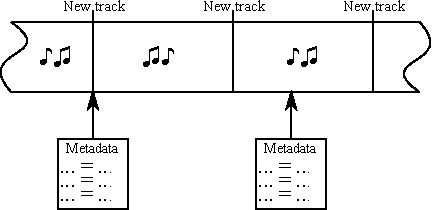
\includegraphics{stream}
  \end{center}
  \fcaption{A \liquidsoap{} stream}
  \label{fig:stream}
  % Stream.png: 500x132 pixel, 91dpi, 14.03x3.70 cm, bb=0 0 398 105
\end{wrapfigure}
A stream can be understood as a timed sequence of data.
In digital signal processing, it will simply be an infinite sequence of 
samples -- floating point values for audio, images for video.
However, multimedia streaming also involves high-level notions.
A \emph{stream}, in \liquidsoap{}, is a succession of \emph{tracks}, annotated
with \textit{metadata}. The tracks can be thought
as individual songs on a musical radio show. 
Metadata are punctual markers storing data, which can occur at any instant in the
stream, and are constituted of a pair of strings consisting of the name of
the metadata and its value. They are used to store various information about the
stream such as copyright information (title or artist of
the current track) or custom information about tracks (for example how loud it
should be played).
Finally, tracks contain data, which consist of float samples 
(for audio data), images (for video data), etc. (see Section~\ref{sec:content}).
A schematic representation of a stream is given in Figure~\ref{fig:stream}.
\TODO{DB Pour une prochaine version, il y a peut etre une remarque plus
  profonde ici. Les autres outils sont des outil de traitement de flux;
  chez eux une source produit un flux. Chez nous, il y a plus de sources
  que de flux à cause du comportement interactive non trivial.

  Par exemple, la fallibilité. C'est une propriété des sources, invisible
  sur les flux. Si on essaie de réparer ça pour revenir à une vision
  plus fonctionnelle, on met des trous dans la notion de flux. Mais ça ne
  marche toujours pas: la taille du trou dans le flux d'une playlist
  dépend de son contexte (avec quoi elle est mise en fallback).

  Un truc marrant c'est qu'on encapsule ces aspects impératifs dans des
  boites noires, pour n'offrir qu'une vision fonctionnelle à 
  l'utilisateur\ldots}

Streams are generated on the fly interactively by operators which are parametrized by various 
external factors (variables possibly modified by external interfaces and metadata in particular).
In \liquidsoap{}, a stream generator is called a \emph{source}. Some sources
purely produce a stream, getting it from an external device (such as a file, a
sound card or network) or are synthesizing it. Many other sources are actually
operating on other sources in the sense that they produce a stream based on input
streams given by other sources. Abstractly, the program describing the
generation of a stream can thus be represented by a directed acyclic graph,
whose nodes are the sources and whose edges indicate dependencies between
sources (an example is given in Figure~\ref{fig:simple}).

% Given an acyclic graph describing a stream generator, the roots of the graph are the operator that create 
% the initial streams, called \textit{sources}. Those sources can be created from a single file, a playlist, an HTTP input,
% the sound card, etc. The sources are then modified and composed with each other using 
% \textit{operators} that, for instance, play a source if it is available or a second one otherwise, or modify
% the metadata, mix the audio data of two sources, etc.
% Finally, the leaves of the graph describe the \textit{outputs} of the stream. Those outputs consist, for instance,
%% DB first occurrence of icecast, never introduced
% of playing the stream on the local sound card, saving it to a file or sending it to and Icecast server. 
% For this initial description, we suppose that the graph has only one output.

Some sources have a particular status: not only do they compute a stream like any
other source, but they also perform some observable tasks, typically outputting
their stream somewhere. These are called \emph{active} sources. Stream
generation is performed ``on demand'': active sources actively attempt to
produce their stream, obtaining data from their input sources which in turn
obtain data from their dependent sources, and so on. An important consequence of
\TODO{DB NON Justement on les crée une seule fois}
this is the fact that \emph{sources do not constantly stream}: if a source would
produce a stream which is not needed by any active source then it is actually
frozen in time.
% DB Technical remark: the source can notice that time still ticks while
%   it is not streaming, but only a few sources use it.
This avoids useless computations, but is also crucial to obtain
the expected expressiveness. For example, a \texttt{rotation} operator will play
alternatively several sources, but should only rotate at the end of tracks, and
its unused sources should not keep streaming, otherwise we might find them in
the middle of a track when we come back to playing them. Likewise, we need to be
able to insert a jingle in between two tracks of a stream, which involves
momentarily stopping it. \emph{Sources are also allowed to fail},
\ie{} refuse to stream at some point in the time at the end of a track (think
for example of a queue of user requests which might often be empty,
or a playlist which takes too long to prepare a file for streaming).

\subsection{A language for building streaming systems}

Based on the streaming model presented above, \liquidsoap{} provides the user
with a convenient high-level language for describing streaming systems.
Although our language borrows from other functional programming languages, it is
has been designed from scratch in order to be able to have a dedicated static
typing discipline together a very user-friendly language. 
\TODO{DB find a better place for technical data?}
It is implemented in OCaml and uses several C libraries 
through external bindings, most of them also developed within the 
\savonet{} project. The code contains approximatively $20$K lines of
OCaml code and $10$K lines of C code and runs on all major operating systems.
% , including Linux, Mac OSX and Windows.
The software along with its documentation is freely
available\footnote{\url{http://savonet.sourceforge.net}} under an open-source
license.

One of the main goals which has motivated the design of the \liquidsoap{}
language is that it should be very accessible, even to non-programmers. It
turned out that having a functional programming language is very natural (\cf
Section~\ref{sec:transitions}). The built-in functions of the language often
have a large number of parameters, many of which have reasonable default 
values, and  it would be very cumbersome to have to write them all each time,
in the right order.
In order to address this, we have designed a new extension of
$\lambda$-calculus with labeled arguments and multi-abstractions which makes it
comfortable to use the scripting
API~\cite{baelde-mimram:webradio-lambda}. Having designed our own language also
allowed us to integrate a few domain-specific extensions, to display helpful
error messages and to generate a browsable documentation of the scripting API. In
practice, many of the users of \liquidsoap{} are motivated by creating a radio
and not very familiar with programming, so it can be considered that the design of
the language was a reasonable success from this point of view.

An other motivation was to ensure some safety properties of the stream
generation. A script in \liquidsoap{} describes a system that is intended to run
for months, some parts of whose rarely triggered, and it would be very
disappointing to notice a typo or a basic type error only after a particular
part of the code is used for an important event. In order to ensure essential
safety properties, the language is statically and strongly typed.
We want to put as
much static analysis as possible, as long as it doesn't put the burden on the
user, \ie{} all types should be inferred. As we shall see, \liquidsoap{} also
provides a few useful dynamic analysis.

\begin{figure}[t]
 \begin{center}
\[
\xymatrix{
  *+[F]{\mathtt{input.http}}\ar[r]&*+[F]{\mathtt{fallback}}\ar[r]&
  *+[F]{\mathtt{normalize}}\ar[r]&
  *+<10pt>[F=:<30pt>]{\mathtt{output.icecast}}\\
  *+[F]{\mathtt{playlist}}\ar[ur]&\\
}
\]
\end{center}
 \fcaption{A simple streaming system}
 \label{fig:simple}
 % Stream.png: 500x132 pixel, 91dpi, 14.03x3.70 cm, bb=0 0 398 105
\end{figure}

The current paper can be read without a prior understanding of the language and
its typing system, a detailed presentation can however be found
in~\cite{baelde-mimram:webradio-lambda}. We simply recall that the evaluation of
a \liquidsoap{} script triggers the construction of various sources, built from
various operators built into the language.
\TODO{DB moche, et "built into" c'est pas builtin\ldots préciser}
For example, the following script defines two elementary sources, respectively 
reading from an HTTP stream and a playlist of files, composed in a fallback 
(\ie{} the playlist is used when the HTTP stream is unavailable or
  interrupted), 
filtered through a volume normalizer, and sent to an Icecast server which 
broadcasts the stream to listeners:
\begin{verbatim}
output.icecast(%vorbis,mount="myradio",
  normalize(fallback([input.http("http://other.net/radio"),
                      playlist("listing.txt")])))
\end{verbatim}
The graph underlying the system resulting from the execution of that script is
shown in Figure~\ref{fig:simple}. A few remarks on the syntax: the notation
\hbox{\texttt{[}\ldots\texttt{]}} denotes a list, \texttt{mount}
is a label (the name of an argument of the function \texttt{output.icecast}) and
\texttt{\%vorbis} is an encoding format parameter whose meaning is explained in
Section~\ref{sec:typing-ex}.

% \subsection{Fallibility}
% 
% \TODO{DB selon la place, on peut envisager de faire sauter cette section;
%   si on la laisse on peut la merger avec la précédente, en plus compact}
% 
% Finally, the information of whether or not a stream can be assumed to be
% infinite is also carried by the graph. For instance, if a source is created from
% a single file, one can try to decode it before starting streaming. If the file
% can be decoded, and one can assume that the file will not be deleted later, and
% then the source can be considered infallible. Later on, if this source is used,
% for instance in an operator that plays the first available source, then the
% source resulting of this operator is also infallible.  By induction over the
% vertices of the graph, each node can be considered fallible or not. Eventually,
% an infallible output can be considered as describing an infinite stream, while a
% fallible output describes a stream that may not be infinite.

\subsection{Efficient frames}
\TODO{DB Benchmark}

An important aspect of the implementation is efficiency concerning both CPU and
memory usage. The streams manipulated can have high data rates (a typical video
stream needs 30Mo/s) and avoiding multiple copies of the data of the streams is
crucial. This is why we use a reference passing mechanism based on frames. A
\emph{frame} is a buffer of data of fixed duration that represents a portion of
the stream. In order to compute a stream, the active sources constantly create
frames and have them filled by passing references to them to their predecessor
sources, which in turn pass the references to their predecessors, and so on.
This passing by reference avoiding copies of data in memory.
% \TODO{DB at this point the reader doesn't see why several frames are needed}
% \TODO{RB I think it is ok now..}

This mechanism is refined in \liquidsoap{} in order to avoid computing twice the
same frame. For instance, one may want to have several outputs of the same
stream, \eg{} one to a server for broadcasting the stream and another one to a
local file for archiving purposes (the circled nodes in
Figure~\ref{fig:sharing}). In this case, the two outputs in the graph are
connected to the same source, and when those outputs transmit their frames to
this source to be filled, the operator should fill them with the same data. In
order to avoid computing the data twice, the first time that the source is asked
to fill a frame, it operates as described before. However, on the second time it
simply fills the frame with the data computed during the first call: computed
frames are \emph{cached} if necessary. \TODO{DB: What about the third time,
  fourth? When does it stop?  We need to talk about clock cycles to avoid
  confusing the reader.}  Once all the filling operations have been done, the
sources are informed that the stream has moved on to the next frame and can
forget their cache. The necessity for a source to cache its current frame is
detected when instantiating the stream generator.
% thus copying data in memory only when it is necessary.
\TODO{DB This paragraph doesn't say much; a little more could be said after
  transitions are evoked.}

\begin{figure}[t]
 \begin{center}
\[
\xymatrix{
  *+[F]{\mathtt{input.http}}\ar[r]&*+[F]{\mathtt{fallback}}\ar[r]&
  *+[F]{\mathtt{normalize}}\ar[r]\ar[dr]&
  *+<10pt>[F=:<30pt>]{\mathtt{output.icecast}}\\
  *+[F]{\mathtt{playlist}}\ar[ur]& & & *+<10pt>[F=:<30pt>]{\mathtt{output.file}}\\
}
\]
\end{center}
\fcaption{A streaming system with sharing}
\label{fig:sharing}
 % Stream.png: 500x132 pixel, 91dpi, 14.03x3.70 cm, bb=0 0 398 105
\end{figure}

\subsection{Functional transitions}
\label{sec:transitions}

\liquidsoap{} is a \emph{functional} programming language and a particularly
interesting application of this is the case of \textit{transitions}, 
\eg{} how two switch from one source to another: do we
want to mix a bit the two sources in order to have a smooth transition? do we
want to add a jingle during the transition? etc. For example, a \emph{crossfade}
consists in mixing the end of the old source, whose volume is faded out, with the
beginning of the new one, whose volume is faded up (see Figure~\ref{fig:cross}).
\vspace{-5ex}
\begin{figure}[h]
 \begin{center}
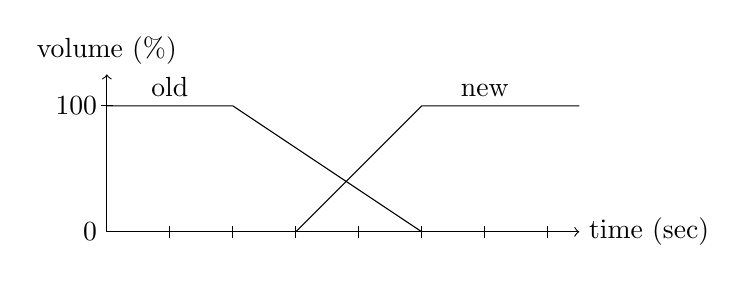
\begin{tikzpicture}[xscale=0.8,yscale=0.8]
\draw[->] (0,0) -- (0,2.5);
\draw (-0.1,2) -- (0.1,2);
\draw (0,2) node[anchor=east]{100};
\draw (0,0) node[anchor=east]{0};
\draw[->] (0,0) -- (7.5,0);
\foreach \x in {1,2,3,4,5,6,7} \draw (\x,-0.1) -- (\x,0.1);
\draw (0,2.5) node[anchor=south]{volume (\%)};
\draw (7.5,0) node[anchor=west]{time (sec)};
\draw (0,2) -- (2,2) -- (5,0);
\draw (3,0) -- (5,2) -- (7.5,2);
\draw (1,2) node[anchor=south]{old};
\draw (6,2) node[anchor=south]{new};
\end{tikzpicture}
\end{center}
 \fcaption{A crossfade transition between two tracks}
 \label{fig:cross}
 % Stream.png: 500x132 pixel, 91dpi, 14.03x3.70 cm, bb=0 0 398 105
\end{figure}

For instance, in \liquidsoap{} the construction \texttt{fallback([$r$,$s$])} interactively
selects between two sources: it fills its frame using the source \texttt{$r$} if
it is available, or the source \texttt{$s$} otherwise.  When switching from
one source to another, it is possible to specify a transition, which is given by
a function whose type is \hbox{\texttt{(source*source)->source}}, \ie{} a
function that takes the two sources as argument, the old and new source, and
return a new source, which gives the transition between them. Thus, the
following code defines a fallback source which performs a crossfade when
switching from one source to another:
\begin{verbatim}
 def crossfade(old,new) =
   add([fade.in(new), fade.out(old)])
 end
 f = fallback(transitions=[crossfade, crossfade], [r, s])
\end{verbatim}

Because any function can be used to define a transition, the possibilities
offered are numerous. For instance, the standard library (programmed in
\liquidsoap{}) defines the operator \texttt{smooth\_add}, which takes as
argument a main source (the tracks of a radio for instance) and a source of
jingles. When a new jingle is available, \texttt{smooth\_add} reduces the volume
of the main source, superposes the jingle to the current track, and increases
the volume of the main track back when the jingle is finished, producing a
dynamic jingle incrustation very easy to use and quite appreciated by
users.
% \footnote{Unfortunately, the code of this function would not fit in the
%   margin. It is available online at this address: \url{http://bit.ly/aHE0G0}}

\section{Heterogeneous stream contents}
\label{sec:content}


% DB les sous-sections peuvent virer, surtout pour faire de la place
%   par contre l'organisation globale doit rester: on raconte ce qu'il
%   se passe au niveau des sources, pour bien montrer que ce qu'on fait
%   dans le typage correspond précisemment aux contraintes imposées
%   par le modele
% \subsection{Model}

% Meme si ya le mot sous-typage, cette relation est vraiment utilisée
% dans le modele indépendamment du langage, d'ailleur c'est
% Frame.kind_sub_kind. Après on copie tout ça au niveau du langage.

In \liquidsoap{}, streams can contain data of various nature. The typical
example is the case of video streams which usually contain both images and
audio samples. We also support MIDI streams (which contain musical notes)
and it would be easy to add other kinds of content.
% which allows us to provide
% ``synthesizer'' operators
% (which take a stream of notes as input and produce an
% audio stream).
% In addition, there can be multiple channels of data for each data
% kind: audio is usually stored in stereo (2~channels), but also sometimes in
% surround sound (5~channels), etc.
It is desirable to allow sources of different
content kinds within a streaming system, which makes it necessary to
introduce a typing discipline in order to ensure 
the consistency of stream contents across sources.
% (\eg some sources might produce sound and other only video and they are merged
% afterward)

The nature of data in streams is described by its \emph{content type}, which is
a triple of natural numbers indicating the number of audio, video and midi
channels.  A stream may not always contain data of the same type.  For instance,
the \texttt{playlist} operator might rely on decoding files of heterogeneous
content, \eg\ mono and stereo audio files.  In order to specify how content
types are allowed to change over time in a stream, we use \emph{arities}, which
are essentially natural numbers extended with a special symbol $\star$:
\[
a\quad ::=\quad \star \;|\; 0 \;|\; S(a)
\]
An arity is \emph{variable} if it contains $\star$, otherwise it is an usual
natural number, and is \emph{fixed}. A \emph{content kind} is a triple of
arities, and specifies which content types are acceptable. For example,
$(S(S(0)),S(\star),\star)$ is the content kind meaning ``2 audio channels, at
least one video channel and any number of MIDI channels''.
% S<:T means "if you can work with T you can work with S"
%            "if you can work with a source(T) you can take a source(S)"
%            "T is more permissive than S"
This is formalized through the subtyping relation defined in
Figure~\ref{fig:subtyping}: $T\sub K$ means
that the content kind $T$ is allowed by $K$. More generally,
$K \sub K'$ expresses that $K$ is more permissive than $K'$,
which implies that a source of content kind $K$ can safely be seen
as one of content kind $K'$.

\begin{figure}[t]
\[
% c'est possible de simplifier en mettant direct K<:K,
% mais on ne peut pas dire K<:* sans vérifier que K est bien formé
   \infer{0\sub 0}{} \quad\quad
   \infer{S(A)\sub S(A')}{A\sub A'} \quad\quad
   \infer{\star\sub\star}{} \quad\quad
   \infer{0\sub \star}{} \quad\quad
   \infer{S(A)\sub \star}{A\sub\star}
\]\[
   \infer{(A,B,C) \sub (A',B',C')}{A \sub A' & B\sub B' & C\sub C'}
\]
 \vspace{-0.3cm}\fcaption{Subtyping relation on arities}
 \label{fig:subtyping}
\end{figure}

When created, sources are given their expected content kind.
Of course, some assignments are invalid.
For example,
a pure audio source cannot accept a content kind which requires video 
channels, and many operators cannot produce a stream of an other kind
than that of their input source.
Also, some sources have to operate on input streams that have a fixed kind --
a kind is said to be fixed when all of its components are.
This is the case of the \texttt{echo} operator which produces echo on sound
and has a internal buffer of a fixed format for storing past sound,
or sound card inputs/outputs which have to initialize the sound card for
a specific number of channels.
Also note that passing the expected content kind
is important because some sources behave differently depending on their kind,
as shown with the previous example.

\label{sec:typing-ex}
\begin{figure}[b]
  \centering
  \texttt{
    \begin{tabular}{rcl}
    swap&:&(source(2,0,0)) -> source(2,0,0)\\
    on\_metadata&:&(handler,source('*a,'*b,'*c)) -> source('*a,'*b,'*c)\\
    % id&(source('a,'b,'c)) -> source('a,'b,'c)\\
    echo&:&(delay:float,source('\#a,0,0)) -> source('\#a,0,0)\\
    % DB vire le prefixe "video." pour faire de la place a gauche
    %  en vrai greyscale veut du fixed arity, pcq son implem est pas
    %  assez générale
    greyscale&:&(source('*a,'*b+1,'*c)) -> source('*a,'*b+1,'*c)\\
    output.file &:& 
       (format('*a,'*b,'*c),string,source('*a,'*b,'*c))->\\
     & & source('*a,'*b,'*c)
    \end{tabular}
  }
  \fcaption{Types for some operators}
  \label{fig:types}
\end{figure}

\paragraph{Integration in the language.}
To ensure that streaming systems built from user scripts will never
encounter situations where a source receives data that it cannot handle,
we leverage various features of our type system.
By doing so, we guarantee statically that content type mismatches never happen.
The content kinds are reflected into types,
and used as parameters of the \texttt{source} type.
In order to express the types of our various operators,
we use a couple features of type systems
(see \cite{pierce02book} for extensive details).
As expected, the above subtyping relation is integrated into
the subtyping on arbitrary \liquidsoap\ types.
We illustrate various content kinds in the examples of Figure~\ref{fig:types}:
\begin{itemize}
\item The operator \texttt{swap} exchanges the two channels of a stereo audio
  stream. Its type is quite straightforward: it operates on streams with exactly
  two audio channels.
\item
  \liquidsoap\ supports polymorphism \emph{à la} ML.
  We use it in combination with constraints to allow arbitrary arities.
  The notation \verb.'*a. stands for a universal variable (denoted
  by \verb.'a.) to which a type constraint is attached, expressing that
  it should only be instantiated with arities.
  For example, the operator \verb.on_metadata. does not rely
  at all on the content of the stream, since it is simply in
  charge of calling a handler on each of its metadata packets --
  in the figure, \verb.handler. is a shortcut for
  \verb.([string*string]) -> unit..
\item When an operator, such as \verb.echo., requires a fixed content type, we
  use another type constraint. The resulting constrained universal
  variable is denoted by \verb.'#a. and can only be instantiated with
  fixed arities.
\item The case of the \texttt{greyscale} operator, which converts a color
  video into greyscale, shows how we can require at least one video channel in
  types.  Here, \verb.'*b+1. is simply a notation for \verb.S('*b)..
\item Finally, the case of \verb#output.file# (as well as several other outputs
  which encode their data before sending it to various media) is quite
  interesting. Here, the expected content kind depends on the format the stream
  is being encoded to, which is given as first argument of the operator. Since
  typing the functions generating formats would require dependent types (the
  number of channels would be given as argument) and break type inference, we
  have introduced particular constants for type formats with syntactic sugar for
  them to appear like functions -- similar ideas are for example used to type
  the \texttt{printf} function in OCaml. For example,
  \verb$output.file(%vorbis,"stereo.ogg",s)$ requires that
  \verb.s. has type \verb.source(2,0,0). because \verb.%vorbis. alone
  has type \verb.format(2,0,0).,
  but \verb$output.file(%vorbis(channels=1),"mono.ogg",s)$
  requires that there is only one audio channel;
  we also have video formats such as \verb.%theora..
\end{itemize}

These advanced features of the type system are statically inferred, which means
that the gain in safety does not add any burden on users. As said above, content
kinds have an influence on the behavior of sources |
polymorphism is said to be \emph{non-parametric}.
In practice, this means that static types must be
maintained throughout the execution of a script. This rather unusual aspect
serves us as an overloading mechanism: the only way to remove content kinds from
execution would be to duplicate our current collection of operators with a
different one for each possible type instantiation.
\TODO{SM c'est pas très clair cette dernière phrase \\
  DB ouais, c'est techniquement dense, j'arrive pas à faire mieux
   mais je vais laisser pour contrer les puristes du parametric polymorphism}

%% SM c'est du détail et on a pas bcp de place
% Type inference leaves unknown types, they are forced using the default
% number of channels, and users can write type annotations.
% But in most cases, type inference works pretty well, since most
% outputs dictate content kinds.


Ideally, we would like to add some more properties to be statically checked by
typing. But it is sometimes difficult to adapt the type system while keeping
nice properties (type inference, principal types, etc.). For example,
\liquidsoap{} checks that active sources are \emph{infallible}, \ie{} always
have data available in their input stream, and this check is currently done by a
flow analysis and not typing. Another example is clocks which are described next
section.


\section{Clocks}
\label{sec:clocks}

Until now, we have only described streaming systems where there is
a unique, global clock. In such systems, time flows at the same rate
for all sources.
% DB I think "wallclock time" is better than "real time" which has 
%    other connotations
By default, this rate corresponds to the wallclock time,
which is appropriate for a live broadcast,
but it does not need to be so.
For example, when producing a file from other files,
one might want the time rate to be as fast as the CPU allows.

\subsection{Motivation}

While having a global clock suffices in many situations,
there are a couple of reasons why a streaming system might involve multiple
clocks or time flows.
The first reason is external to liquidsoap: there is simply
not a unique notion of time in the real world.
A computer's internal clock indicates a slightly different time
than your watch or another computer's clock.
Moreover, when communicating with a remote computer, network
latency causes a perceived time distortion.
Even within a single computer there are several clocks: notably, each
soundcard has its own clock, which will tick at a slightly different
rate than the main clock of the computer.
Since liquidsoap communicates with soundcards and remote computers,
it has to take those mismatches into account.

There are also some reasons that are purely internal to liquidsoap:
in order to produce a stream at a given speed,
a source might need to obtain data from another source at
a different rate. This is obvious for an operator that speeds up or
slows down audio, but is also needed in more subtle cases
such as a crossfading operator.
\TODO{SM on devrait déjà avoir expliqué le crossfading avant}
Crossfading consists in fading the volume of a stream around tracks
limits, which is not problematic, and more crucially combining a portion
of the end of a track with the beginning of the next one\footnote{
  In \liquidsoap, crossfading derives from a simpler operator that
  only takes care of crossing, \ie\ combining the end of a track
  with the beginning of the next one. The \texttt{cross} operator
  takes a transition function as a parameter for describing how
  the two tracks are actually combined.
}.
\TODO{SM 1. c'est pas joli les notes 2. est ce que celle-ci n'est pas trop du détail ?}
The result is close to what was represented in Figure~\ref{cross-fig}
except that the two tracks originate from the same source.
During the lapse of time where the operator combines
data from an end of track with the beginning of the other other,
the crossing operator needs twice as much stream data\footnote{
  % Note that there is no need to store the beginning of track
  % (this is only done in smart_cross for computing its volume)
  In the actual implementation, we have to
  maintain a copy of a section of the past content
  of the input stream until the end of a track,
  generally using remaining time estimations to avoid maintaining
  this sliding window all the time.
  The time acceleration does not actually happen
  when the tracks are combined but when the sliding window
  is initially filled up.
}.
\TODO{SM pareil, c'est trop implém}
After ten tracks,
with a crossing duration of six seconds, one more minute will have
passed for the source compared to the time of the crossing operator.

\subsection{Model}

In order to avoid inconsistencies caused by time differences,
while maintaining a simple and efficient execution model for
its sources, liquidsoap works under the restriction that
one source belongs to a unique clock,
fixed once for all when the source is created.
Sources from different clocks cannot communicate using the normal
streaming protocol, since it is organized around clock cycles.
Each clock is responsible for animating its own active sources
and has full control on how it does it.

In the graphical representation of streaming systems,
clocks induce a partition of sources represented by a notion of locality
or box, and clock dependencies are represented by nesting.
For example, the graph shown in Figure~\ref{fig:boxes}
corresponds to the stream generators built in the following
script:
\begin{verbatim}
output.icecast(%vorbis,mount="myradio",
  fallback([crossfade(playlist("some.txt")),jingles]))
\end{verbatim}

\begin{figure}[t]
 \begin{center}
\[
\def\f{\save
*+<15pt>[F--]\frm{}\ar @{--} "2,2"\restore}%
\def\g{\save
"2,4"."1,2"."1,5"!C*+<27pt>[F--]\frm{}\ar @{--} "1,1"\restore}%
\xymatrix{
   \mathtt{clock_1} & *+[F]{\mathtt{playlist}}\ar[r]\f&*+[F]{\mathtt{crossfade}}\ar[r]&  *+[F]{\mathtt{fallback}}\ar[r]&
  *+[F]{\mathtt{output.icecast}}\\
   &\mathtt{clock_2} &  & *+[F]{\mathtt{jingles}}\ar[u]\g& 
}
\]
\end{center}
 \caption{A streaming system with two clocks}
 \label{fig:boxes}
 % Stream.png: 500x132 pixel, 91dpi, 14.03x3.70 cm, bb=0 0 398 105
\end{figure}

There, $\verb.clock._{\tiny{\verb.2.}}$
was created specifically for the crossfading
operator; the rate of that clock is controlled by that operator,
which can hence accelerate it around track changes without any
risk of inconsistency.
The other clock is simply a wallclock, so that the main stream
is produced following the real (wallclock) time rate.

A clock is said to be active if it ticks by itself,
therefore running its sources constantly.
It is the case of wallclocks or soundcard clocks.
We say that a clock depends on another one
if its animation (and thus time rate) depends on it.
% DB: I wanted to write this since it holds geometrically for nesting
%   "It is not possible for a clock to depend (directly) on several others."
%   but it doesn't seem forced by anything,
%   and in fact the implementation should allow it
Active sources do not depend on other sources,
and dependencies must be acyclic.
In the above example, the ticking of
$\verb.clock._{\tiny{\verb.2.}}$ is provoked by that of
$\verb.clock._{\tiny{\verb.1.}}$, and freezes when the fallback
is playing jingles.
% a clock $c'$ might depend on $c$ if it ticks twice as fast;
% such a clock will be used in the implementation of a speed doubling
% operator.
Although nothing forces it in the model, it makes more sense if
each passive source depends (possibly indirectly) on an active one,
and all sources without dependencies are active.
Those assumptions are in fact guaranteed to hold for the systems
built from the \liquidsoap\ language.
% this is because the user only creates wallclocks
% and the only dependent clocks are suitably nested (cross and stretch)

From an implementation viewpoint, each active clock launches
its own streaming thread.
Hence, clocks provide a way to split the generation of one or
several streams accross several threads,
and hence multiple CPU cores\footnote{
  Although OCaml uses a global memory management lock that makes it
  impossible for two OCaml threads to run concurrently, there is no
  such constraint when a thread runs a foreign function.
  This allows us to avoid the limitation since
  most of the computation in \liquidsoap\ takes place in decoding
  and encoding multimedia formats, which is done by C libraries.
}.
This powerful possibility is made available to the user
through the intuitive notion of clock.
As we shall see in the next section,
the script writer never needs to specify clocks unless he
explicitly wants a particular setup,
and \liquidsoap\ automatically checks that clock assignements
are correct.

\TODO{DB: should we show the nice example from the doc where icecast
  does not interfere with a file backup and a sound card input?
  Perhaps just mention it above, but some code could be nice.}

\subsection{Clock assignment}

Clocks are not represented in the type of \liquidsoap\ sources.
Although it would be nice to statically check clock assignment,
type inference would not be possible without technical annotations
from the user.

Instead, clocks are assigned upon source creation.
Some sources require to belong to a particular, definite clock,
such as the wallclock, or the clock corresponding to a sound card.
Most sources simply require that their clock is the same as their
input sources.
Since clocks often cannot be inferred bottom-up, we use a notion
of clock variable that can be left undefined.
Clock variables reflect the required clock dependencies,
which are maintained during the inference process.

Two errors can occur during this phase.
Although they are runtime errors that could be raised
in the middle of streaming when new sources are created
(\eg\ by means of a transition),
this usually only happens during the initial construction.
The first error is raised when
two different known clocks need to be unified.
For example, in the following script, the ALSA input is
required to belong to the ALSA clock and \verb.crossfade.'s internal clock
at the same time:
\begin{verbatim}
output.file(%vorbis,"record.ogg",crossfade(input.alsa()))
\end{verbatim}
The other possible error happens when unifying two unknown clock variables
if one depends on the other | in unification terminology, this is an occurs
check failure. A simple example of that situation is
the script \verb.add([s,crossfade(s)]). where the two mixed sources
respectively have clocks $c$ and $X_c$ where $c$ is the clock created
for the crossfading operator and $X_c$ is the variable representing
the clock to which the crossfading belongs, on which $c$ depends.

After this inference phase, it is possible that some clocks are still
unknown. Remaining variables are thus forcibly assigned to the default
wallclock, before that all new sources are prepared for streaming
by their respective clocks.


\section{Related work}

\liquidsoap{} is obviously different from classical tools
such as Ices or Darkice in
that it offers the user the freedom to assemble a stream
for a variety of operators, through a scripting
language rather than traditional configuration files.

\liquidsoap{} has more similarities with multimedia streaming libraries
such as GStreamer~\cite{gstreamer} and digital signal processing (DSP) languages
such as Faust~\cite{faust}.
GStreamer defines a model of stream, and its API
can be used to define streaming systems in various programming
languages (primarily coded in C, the library has also been
ported to many other languages).
Faust~\cite{faust} provides a high-level functional programming language for
describing stream processing devices,
and compiles this language down to C++, which enables an integration
with various other systems.
It is also worth mentioning Chuck~\cite{chuck}, a dynamic language with similar 
views as Faust.
By provinding a higher-level API, \liquidsoap{} differs
from this tools in the following ways: (1) Its operators are simple and 
hide most of the technicalities. (2) The streams created by
\liquidsoap{} contain additional notions, namely tracks and 
metadata. (3) Streams in \liquidsoap are meant for interactive
streaming. In particular, they can be stoped temporarily
or created and destroyed dynamically.
\TODO{DB unlike faust, liquidsoap is interpreted}
It would be very interesting to interface \liquidsoap{} with such tools,
or import some of their techniques.
This could certainly be done with DSP operators, and would allow us to program them efficiently 
from the scripting language rather than in OCaml.
Finally, \liquidsoap{} has been used in research~\cite{baccigalupo2007case,baccigalupo2007sharing},
in order to study the social aspects of web radios.


\TODO{has been used in research~\cite{baccigalupo2007case,baccigalupo2007sharing}}
\TODO{on peut citer, je sais pas où, mais j'insisterais pas sur
  l'utilisation en recherche (c'est une utilisation comme une autre,
la recherche de claudio est indépendante de liq)}
\TODO{RB En même temps ça vaut quand même le coup de le mentioner. Par exemple
dans related work..}

\section{Conclusion}

Documentation, errors, user friendliness.
Requests.
Typing sources as objects whose methods are (telnet) services.

\TODO{SM 4 papiers ça fait vraiment très léger comme biblio, faudrait en rajouter}
\bibliographystyle{abbrv}
\bibliography{biblio}
\end{document}
